%%%%%%%%%%%%%%%%%%%%%%%%%%%%%%%%%%%%%%%%%
% Programming/Coding Assignment
% LaTeX Template
%
% This template has been downloaded from:
% http://www.latextemplates.com
%
% Original author:
% Ted Pavlic (http://www.tedpavlic.com)
%
% Note:
% The \lipsum[#] commands throughout this template generate dummy text
% to fill the template out. These commands should all be removed when 
% writing assignment content.
%
% This template uses a Perl script as an example snippet of code, most other
% languages are also usable. Configure them in the "CODE INCLUSION 
% CONFIGURATION" section.
%
%%%%%%%%%%%%%%%%%%%%%%%%%%%%%%%%%%%%%%%%%

%----------------------------------------------------------------------------------------
%	PACKAGES AND OTHER DOCUMENT CONFIGURATIONS
%----------------------------------------------------------------------------------------

\documentclass{article}

\usepackage{fancyhdr} % Required for custom headers
\usepackage{lastpage} % Required to determine the last page for the footer
\usepackage{extramarks} % Required for headers and footers
\usepackage[usenames,dvipsnames]{color} % Required for custom colors
\usepackage{graphicx} % Required to insert images
\usepackage{listings} % Required for insertion of code
\usepackage{courier} % Required for the courier font
\usepackage{lipsum} % Used for inserting dummy 'Lorem ipsum' text into the template

% Margins
\topmargin=-0.45in
\evensidemargin=0in
\oddsidemargin=0in
\textwidth=6.5in
\textheight=9.0in
\headsep=0.25in

\linespread{1.1} % Line spacing

% Set up the header and footer
\pagestyle{fancy}
\lhead{\hmwkAuthorName} % Top left header
\chead{\hmwkClass\ (\hmwkClassInstructor\ \hmwkClassTime): \hmwkTitle} % Top center head
\rhead{\firstxmark} % Top right header
\lfoot{\lastxmark} % Bottom left footer
\cfoot{} % Bottom center footer
\rfoot{Page\ \thepage\ of\ \protect\pageref{LastPage}} % Bottom right footer
\renewcommand\headrulewidth{0.4pt} % Size of the header rule
\renewcommand\footrulewidth{0.4pt} % Size of the footer rule

\setlength\parindent{0pt} % Removes all indentation from paragraphs

%----------------------------------------------------------------------------------------
%	CODE INCLUSION CONFIGURATION
%----------------------------------------------------------------------------------------

\definecolor{MyDarkGreen}{rgb}{0.0,0.4,0.0} % This is the color used for comments
\lstset{language=C++,
	basicstyle=\ttfamily,
	keywordstyle=\color{blue}\ttfamily,
	stringstyle=\color{red}\ttfamily,
	commentstyle=\color{MyDarkGreen},
	morecomment=[l][\color{magenta}]{\#}
}

% Creates a new command to include a perl script, the first parameter is the filename of the script (without .pl), the second parameter is the caption
\newcommand{\perlscript}[2]{
\begin{itemize}
\item[]\lstinputlisting[caption=#2,label=#1]{#1.cpp}
\end{itemize}
}

%----------------------------------------------------------------------------------------
%	DOCUMENT STRUCTURE COMMANDS
%	Skip this unless you know what you're doing
%----------------------------------------------------------------------------------------

% Header and footer for when a page split occurs within a problem environment
\newcommand{\enterProblemHeader}[1]{
\nobreak\extramarks{#1}{#1 continued on next page\ldots}\nobreak
\nobreak\extramarks{#1 (continued)}{#1 continued on next page\ldots}\nobreak
}

% Header and footer for when a page split occurs between problem environments
\newcommand{\exitProblemHeader}[1]{
\nobreak\extramarks{#1 (continued)}{#1 continued on next page\ldots}\nobreak
\nobreak\extramarks{#1}{}\nobreak
}

\setcounter{secnumdepth}{0} % Removes default section numbers
\newcounter{homeworkProblemCounter} % Creates a counter to keep track of the number of problems

\newcommand{\homeworkProblemName}{}
\newenvironment{homeworkProblem}[1][Section \arabic{homeworkProblemCounter}]{ % Makes a new environment called homeworkProblem which takes 1 argument (custom name) but the default is "Problem #"
\stepcounter{homeworkProblemCounter} % Increase counter for number of problems
\renewcommand{\homeworkProblemName}{#1} % Assign \homeworkProblemName the name of the problem
\section{\homeworkProblemName} % Make a section in the document with the custom problem count
\enterProblemHeader{\homeworkProblemName} % Header and footer within the environment
}{
\exitProblemHeader{\homeworkProblemName} % Header and footer after the environment
}

\newcommand{\problemAnswer}[1]{ % Defines the problem answer command with the content as the only argument
\noindent\framebox[\columnwidth][c]{\begin{minipage}{0.98\columnwidth}#1\end{minipage}} % Makes the box around the problem answer and puts the content inside
}

\newcommand{\homeworkSectionName}{}
\newenvironment{homeworkSection}[1]{ % New environment for sections within homework problems, takes 1 argument - the name of the section
\renewcommand{\homeworkSectionName}{#1} % Assign \homeworkSectionName to the name of the section from the environment argument
\subsection{\homeworkSectionName} % Make a subsection with the custom name of the subsection
\enterProblemHeader{\homeworkProblemName\ [\homeworkSectionName]} % Header and footer within the environment
}{
\enterProblemHeader{\homeworkProblemName} % Header and footer after the environment
}

%----------------------------------------------------------------------------------------
%	NAME AND CLASS SECTION
%----------------------------------------------------------------------------------------

\newcommand{\hmwkTitle}{Programming Test} % Assignment title
\newcommand{\hmwkDueDate}{Monday,\ March\ 27,\ 2017} % Due date
\newcommand{\hmwkClass}{U-Play} % Course/class
\newcommand{\hmwkClassTime}{8:30am} % Class/lecture time
\newcommand{\hmwkClassInstructor}{BlueByte - Uplay} % Teacher/lecturer
\newcommand{\hmwkAuthorName}{Nick Houghton} % Your name

%----------------------------------------------------------------------------------------
%	TITLE PAGE
%----------------------------------------------------------------------------------------

\title{
\vspace{2in}
\textmd{\textbf{\hmwkClass:\ \hmwkTitle}}\\
\normalsize\vspace{0.1in}\small{Due\ on\ \hmwkDueDate}\\
\vspace{0.1in}\large{\textit{\hmwkClassInstructor\ \hmwkClassTime}}
\vspace{3in}
}

\author{\textbf{\hmwkAuthorName}}
\date{} % Insert date here if you want it to appear below your name

%----------------------------------------------------------------------------------------

\begin{document}

\maketitle

%----------------------------------------------------------------------------------------
%	TABLE OF CONTENTS
%----------------------------------------------------------------------------------------

%\setcounter{tocdepth}{1} % Uncomment this line if you don't want subsections listed in the ToC

%\newpage
%\tableofcontents
\newpage

\section{Introduction}
The \textit{Acme Elevators} challenge was a fun and interesting challenge. 
This report will be an attempt to describe my thought process and procedure while working towards a solution.
What follows will be a step by step recording of what took place.

\subsection{Preparation}
When the \textit{Acme Elevators} challenge was received the first step I took was to organize the given code into a visual studio project.
Being a windows user I've found Visual Studio (VS) to be one of the most enjoyable C++ development tools.
The new project was included along side a series of other projects of a similar nature for which I have a github repository for safe keeping and version control.\newline

Once the project was set up I began reading through the code however I found the formatting to be unfamiliar.
I spent some time doing some simple rearranging to put the received code into a more familiar and comfortable format.
Once finished I returned to carefully re-reading the problem statement and getting familiar with the code. 

\subsection{Implementation}
Once I had reviewed the incomplete code several times I made a list of all of the locations of the ``Implement Me'' comment.
I then added a \textit{TODO} keyword to each so I could easily track them using visual studio's Track List feature.
As I progressed through implementing the missing code I added a 'Done' tag to each \textit{TODO} comment.

\subsubsection{Elevator}
Once I became familiar with the code structure I began looking at the \textit{Elevator} class since it seemed the most 'low-leveled' in the class structure.
I quickly noticed that it was missing a member which kept track of the destination floor of the elevator instance; I could not see a logical way of directing elevators without one.
With this additional member variable the remaining implementation was relatively straightforward.
Additionally, I noticed that there was no clear definition of number value was used to indicate the bottom floor.
In North American culture the ground floor is commonly referred to as the 'first' floor however in Europe it is commonly floor zero.
I added a simple get method in Utils.h where the ground floor value can be set and retrieved.\newline

It seemed that the easiest way to determine whether an elevator has work to do was whether its current floor equals its target floor.
Theoretically, should these equal the elevator is idle.
The step function seemed to need to only modify the current floor value by one on each iteration.
Assuming the elevator 'HasWork' a check is enacted to ensure it does not go outside of its bounds.
Finally, to select a floor a simple check needed to be done to ensure that the selected floor was attainable by the current elevator. 
Should it be out of range an error message is printed to the standard error stream.


\subsubsection{Elevators}
The \textit{Elevators} class proved to be slightly more confusing at first.
The intended purpose of the ``OnMessageElevatorCall'' and ``OnMessageElevatorRequest'' methods was a little vague at first however I surmised the following:
\begin{itemize}
	\item \textbf{OnMessageElevatorCall}: A human standing in the lobby presses either the ``up'' or ``down'' button to call an elevator to take them in a certain direction.
	\item \textbf{OnMessageElevatorRequest}: A human has entered the elevator and selects a desired floor.
\end{itemize}
I based these interpretations off of the contents of the message objects sent to each. 
The members of the ``MessageElevatorCall'' and ``MessageElevatorRequest'' classes seemed to fit this interpretation well.\newline

Following these definitions, the ``OnMessageElevatorRequest'' method was relatively straightforward to implement. 
It simply needed to search the vector of elevators, find the requested instance and set its target floor value via the ``SelectFloor'' method.\newline

The ``OnMessageElevatorCall'' method was considerably more complicated. 
My initial thought was that this method should populate a queue data structure.
As humans arrive in the lobby to call an elevator the messages should be prioritized and acted upon in the order they arrived. 
However, it came to mind that the not all messages can be serviced immediately.
As an example, if there is only a single elevator, currently on the 4th floor headed towards the 8th floor it is able to stop at any floor in between to pick up additional passengers.
A request from a floor below will not be serviceable as the elevator is traveling away from the call source.
In this scenario, a call from the second floor will need to wait until the elevator completes its current objective and returns to an idle state. 

To implement this a queue which allows entries in the middle of the queue to be removed is needed.
The STL Queue container does not allow this so a Vector was used.
At every ``Step'', the \textit{Elevators} class iterates through the vector from oldest to newest and services (as well as removes from the list) any call it is able to service.\newline

The elevators class must accurately asses the state of all elevators and make a decision which messages are serviceable and how best to do so.
A call to a method named ``ServiceElevatorCalls'' was added to the elevator step method before the step loop to assess calls.
This method calls another method named ``canService'' on each message to determine if that message can be service.
The ``canService'' method is relatively complex as the best decision for the current message needs to be made.
The method loops through each elevator object and evaluates only those that are idle.
Non-idle elevators are currently servicing another request and should not be altered.
To decide which idle elevator is best to service the request a series of conditions are determined:
\begin{itemize}
	\item The current distance away from the calling human.
	\item Whether the elevator is currently above or below the calling floor.
	\item Whether the person wants to go up or down.
	\item Whether the person is on the extremity of the elevators shaft (bottom or top floor).
	\item Whether the requesting floor is reachable by the current elevator.
\end{itemize} 
If the calling floor is not reachable by the current elevator then it obviously can not be considered and is skipped.
The remaining four conditions are evaluated using a boolean logic equation.
A small java application named \textit{Truth-Table Solver} was used to convert a truth table to the desired boolean formula.
As can be seen in Figure~\ref{fig:untitled} the truth table was filled, the solver was then able to compute a sum of products formula.
Any elevator which meets the desired conditions is considered as a candidate to service the incoming call.
A temporary distance variable is used to track the nearest elevator which meets the conditions.\newline
\begin{figure}
	\centering
	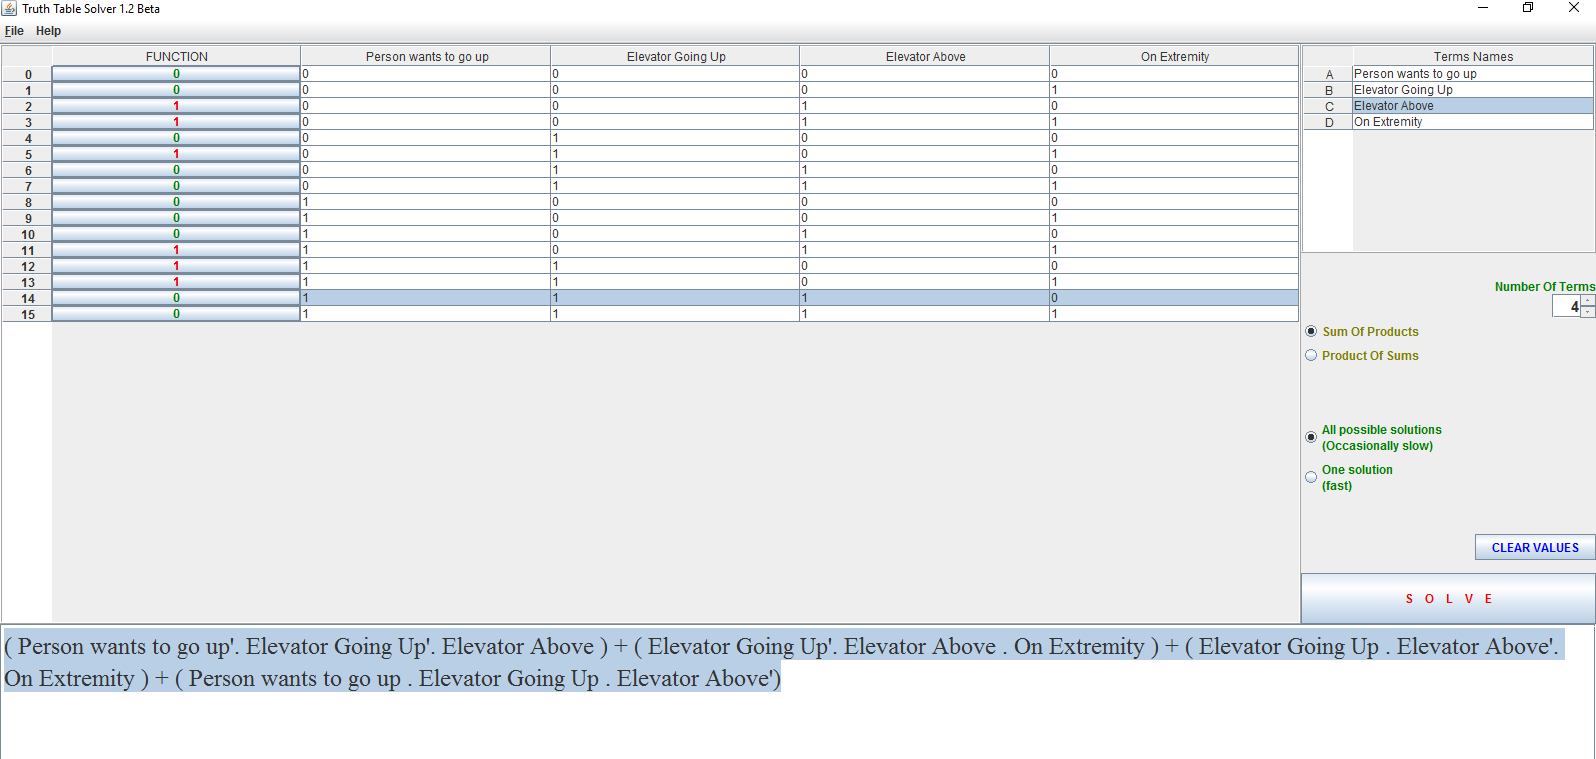
\includegraphics[width=1\linewidth]{Untitled}
	\caption[Truth Table Solver Use]{Truth Table Solver Use}
	\label{fig:untitled}
\end{figure}

The methodology described to select the best elevator relies on some complex logic. 
A unit test using the ``Catch'' C++ unit testing framework was used to verify the logic's validity.
The initial test case for the ``CanService'' method can be seen in Listing~\ref{lst:testCase}.
\begin{lstlisting}[float,caption={Can Service Test Case},xleftmargin=.15\textwidth,label={lst:testCase}]
TEST_CASE("Can Service") {
	Elevators elev;
	std::vector<Elevator>	myElevators;
	
	// Test idle elevators
	myElevators.push_back(Elevator{ 1, 10, 6, Direction::Down });
	elev.setElevators(myElevators);
	MessageElevatorCall mTrue1, mTrue2, mTrue3;
	mTrue1.myDirection = Direction::Up;
	mTrue1.myFloor = 1;
	mTrue2.myDirection = Direction::Down;
	mTrue2.myFloor = 7;
	mTrue3.myDirection = Direction::Up;
	mTrue3.myFloor = 7;
	
	REQUIRE(elev.canService(mTrue1) == true);
	myElevators.clear();
	elev.setElevators(myElevators);
	myElevators.push_back(Elevator{ 1, 10, 6, Direction::Down });
	elev.setElevators(myElevators);
	REQUIRE(elev.canService(mTrue2) == true);
	myElevators.clear();
	elev.setElevators(myElevators);
	myElevators.push_back(Elevator{ 1, 10, 6, Direction::Down });
	elev.setElevators(myElevators);
	REQUIRE(elev.canService(mTrue3) == true);
	
	myElevators.clear();
	elev.setElevators(myElevators);
	
	
	// Test Moving Elevators
	Elevator movingElev(1, 10, 1, Direction::Down);
	movingElev.setTargetFloor(10);
	myElevators.push_back(movingElev);
	elev.setElevators(myElevators);
	
	MessageElevatorCall mTrue4, mFalse1;
	
	mTrue4.myDirection = Direction::Up;
	mTrue4.myFloor = 4;
	mFalse1.myDirection == Direction::Down;
	mFalse1.myFloor = 4;
	REQUIRE(elev.canService(mTrue4) == true);
	REQUIRE(elev.canService(mFalse1) == false);
}
\end{lstlisting}
Several other test cases for the \textit{Elevators} class methods were added but will not be included in this report.

\subsubsection{Humans}
The \textit{Humans} class required only two methods to be implemented.
I began by working on the ``OnMessageElevatorArrived'' method.
I gathered that there were only two cases for which this method should be called:
\begin{enumerate}
	\item When an elevator arrives to pick up a human.
	\item When an elevator reaches its destination to drop off a human.
\end{enumerate}

Knowing these two cases, simple checks can be easily implemented.
When an elevator arrived message is received it must be checked against all humans.
For each human the two conditions listed above are checked.
If a person is in the waiting state and the elevator has arrived to their floor, that person transitions to the traveling state and the elevator becomes occupied.
Currently, only one person can ride in an elevator at a time.
Hopefully this will be remedied later.
When a person is picked up a ``MessageElevatorRequest'' message is generated and broadcast to the elevators.
This emulates the notion that the person has boarded the elevator and has selected a destination floor.\newline

In the case where the person is in the traveling state and the elevator has arrived to their destination floor, the second case stated above has been met.
The human transitions to the arrived state.

The ``OnMessageHumanStep'' method only required handling the cases where a new human arrives and the removal of humans who have completed their journey.
When a human is created the constructor sets the state to ``HumanState\_Idle''. 
The step method looks for humans in the vector with this state. 
If found the a call is made to the elevators and the humans state is changed to ``HumanState\_Waiting''.
A test case was added for the ``OnMessageElevatorArrived'' method to ensure proper function.
Once all of the test cases passed the entire system could be run for the first time.
A test case was not implemented for the human ``OnMessageHumanStep'' because it was the last of the implementations needing completion; it could be tested by running the entire system.

\subsubsection{First-Run}
When run for the first time some issues were quickly discovered.
In the \textit{Elevators} class, the ``canService'' method was not properly discerning between idle and active elevators.
Secondly, a case was not implemented for when a human arrives and an elevator was already on their floor. 
These two bugs were found and easily remedied.
To test the system the initial set up of one elevator and one human was run.
Some additional code was added to the ``OnMessageHumanStep'' method; when a human arrives and is removed from the ``myHumans'' vector a new human was generated randomly.
This allowed the \textit{Elevators} class to run continuously, handling calls and requests as they came in.
They system ran successfully handling each new human who arrived.

\subsection{Increased Number of Humans}
To ramp up the abilities of the system an additional human was added to the ``Humans::Start'' method.
This immediately showed a flaw; when the first human arrived at their destination the elevator was not being rerouted to pickup the second human.
This issue was caused by the ``canService'' method.
When an elevator arrived at the location to pick up the first passenger it caused the ``HasWork'' method to return false because the target and current floors were equal.
This made the \textit{Elevators} class think that it could remove the second passengers call from the queue. 
This was incorrect as there was no elevator to service the second call.
Once the elevator has finished with the first passenger it checked the queue to find it empty.

A solution to this was found by adding an ``onCall'' and ``onRequest'' flag to the \textit{Elevator} class.
This allowed a check to be implemented to prevent the call queue from being modified when there is no elevator to service the message.

\subsection{Increased number of elevators} 
When increasing the number of elevators, if the max floor value were all equal the system worked.
When elevators with different floor counts were created there was an issue with the ``OnMessageElevatorArrived'' and ``OnMessageElevatorRequest'' methods.
When an elevator arrives it sends a ``MessageElevatorArrived'' object. 
This object only contains the elevatorId and the floor it has arrived to.
There is no indication of the maximum floor this elevator can reach.
In the ``OnMessageElevatorArrived'' method, a human uses the elevator that has arrived to their floor.
Once inside, they find there is no way to get to their floor. 
This causes an issue as the human never reaches their destination.
The only solution which could be found at the time was to add an additional parameter to the ``MessageElevatorArrived'' class.
A human would only get on the elevator if the available one was able to reach their destination.\newline

This presented a second issue.
Which elevator would service a call was based upon its availability and its proximity to the human who made the call.
This decision is not based off of the end destination of the user; it can't be as the destination buttons are within the car of the elevator.
The consequence is that when an elevator arrives to service a human who wants to go out of the range of that elevator it is now both on the same floor as the human and available.
All other elevators (who may be able to service the human) are further away.
Since it is not desirable to add a destination variable to the ``MessageElevatorCall'' class an alternative is needed.
The best solution is, when a call is made by a human, all elevators who do not have work will have their target floor set to the calling humans floor.
This way, all available elevators will begin to travel towards the waiting human.
It was realized that the implementation for this issue was left as a bonus, if there is time it will hopefully be addressed.

Further, an additional bug was found in the ``canService'' method.
Elevators that began on a floor which already had a call from a human were not having their ``onRequest'' value set properly.
The consequence of this was that they would complete their first human then never pick up another.
This was quickly remedied with a simple call to the ``setOnRequest'' method.

\subsection{Code Clean-up And Optimization}
Donald Knuth, winner of the 1974 Turing award once said that ``premature optimization is the root of all evil''.
This a sound philosophy which often makes development considerably more enjoyable when followed.
Once the system was working relatively well it was reviewed for performance and cleanliness.
Additional comments were added and unit tests were used to ensure proper functionality was maintained.
By this point of the challenge the 48 hours was running low; code can almost always be better.
The following is a list of general C++ code facets which were used to ensure a better performance.
\begin{itemize}
	\item Use of prefix operators over postfix.
	\item Use of constructor initialization lists.
	\item Parameters passed by reference where possible.
\end{itemize} 

\section{Discussion}

\subsection{Unit Tests}
Each of the unit tests have been commented out and moved to the bottom of the .cpp file of their respective classes.
These tests employ the ``Catch'' framework's TEST\_CASE macro which require the catch\_main function to run.
The catch\_main is a main class within the ``Catch'' framework; when it and the system's main function are both present they are considered overloaded which, of course is not allowed.
To run the test cases they must be uncommented.
The main method for the system in main.cpp must be commented out to allow the catch\_main to run.
Finally, at the top of there is a ``\#define CATCH\_CONFIG\_MAIN'' commented out at the top of main.cpp.
This as well must be uncommented to run the test cases.
\subsection{TODO List}
Throughout development the TODO task list feature of visual studio was used extensively.
These comments were intentionally left within the source code to give the reviewer a sense of the thought process during development.
\subsection{Bonus Questions}

\subsubsection{Thread Class Enhancement}
The current implementation of the threads relies on a timing construct to update the state of the elevators and humans.
Since elevators take time to move their progress should still be based on time however the processing of input from users and elevators should not be delayed while waiting for the step methods to be run.
Ideally the worker threads would sleep on their respective condition variables, waiting from input from other entities.
They currently sleep until a predefined time and then wake to possibly do nothing.
Both the \textit{Elevators} and \textit{Humans} classes should be given methods which send receive signals via the condition variables.

\subsubsection{Clean Exit}

\subsubsection{Different Sized Buildings}
During development it was not realized that this feature was a bonus question. 
An attempt was made to implement a system such that the elevators could have a variable number of floors.
This would emulate a building where a the primary elevator can not access the penthouse suite while a second secret elevator can.
It quickly became apparent that the current code would need some restructuring in order to allow this feature.
First, the messages passed between the human an elevator worker threads would need to change slightly.



\end{document}